%!TEX root = paper.tex
%%%%%%%%%%%%%%%%%%%%%%%%%%%%%%%%%%%%%%%%%%%%%%%%%%%%%%%%%%%%%%%%%%%%%%%%%%%%%%%%
\section{An End-to-End Lag Model}
\label{sec:model}

\begin{figure*}[!t]
	\centering
	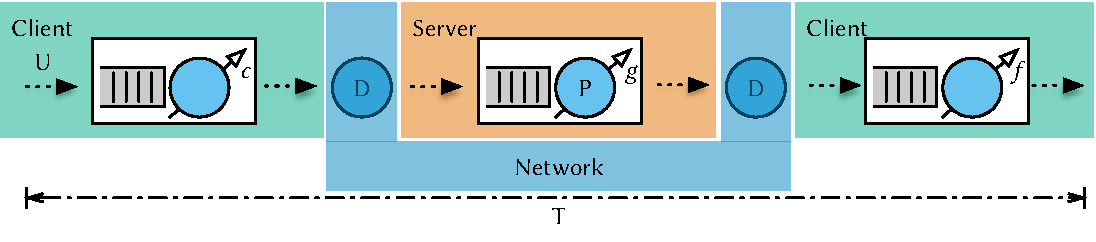
\includegraphics[width=0.9\textwidth]{../../../models/e2e-lag-model.pdf}
	\caption{Queuing lag model in an online video game case.}
\label{fig:queuing-model}
\end{figure*}

The \gls{E2E} lag $T$ can be defined as the elapsed time between a player inputting some commands and the results of these commands being displayed on screen. The section describes this lag as a model for the case of an online dedicated client/server game. The player input is assumed to be a stochastic process $U$. Furthermore, input events are queued up and sent en bloc at specific intervals defined by the command rate $c$. A fixed tickrate $g$ is associated with the computation process of the game server, and a framerate $f$ with the rendering process. The server updates the state of the game world at every tick, and may spend some processing time $P \leq \frac{1}{g}$ in order to do so. The processing time is a random variable which is assumed to follow a truncated normal distribution in our simulations. Once finished, an update message is sent to the client. The contents of this update message can then only be incorporated into the next rendering cycle and not the one that is currently in progress. While the rates of the command, tick, and render cycles are assumed to be constant for the sake of this model (though not necessarily identical), they are not operating in lockstep but independently of each other. This is represented in the model by a random initial phase offset for each rate. Since the model's focus is on depicting an online game, it includes the network paths between the different entities. A random variable $D$ represents the networking delay between game client and server. Fig.~\ref{fig:queuing-model} gives a graphical representation of the queuing model for the online video game case, especially including the three clocked processes responsible for the game's interactions.

The model for cloud gaming is slight variation of this online game model, adapting its notions of $D$, $P$, $T$, $U$, $c$, and $f$. However, the server now handles only one client, and becomes a \textit{streaming server} that also renders and encodes the screen contents, adding a constant encoding delay $e$. On the client side, the stream is decoded (adding decoding delay $d$) before being displayed.


\subsection{Model Limitations}

These models do not attempt to capture all possible sources of lag that occur in actual gaming. Indeed, the models simplify the following aspects in the hope to make the results more tractable. First, the models ignore the delays contributed by input devices like keyboards, mice, and game controllers, estimated to be below \SI{10}{\milli\second}. The same goes for the lag of the display device which is typically in the range of \SIrange{9}{40}{\milli\second} for a PC monitor, and often larger for TVs. The models can be extended to take those delay factors into account, but they were exempted for the sake of simplicity in this paper. Modern games go to great lengths to handle lag gracefully, and try to ``work around it'' in various ways. The methods for this vary, and implementations usually are not easy to examine, providing a good opportunity for future work. Such techniques can typically be subsumed under the term ``lag compensation'', e.g., the game client tries to predict the server state from past knowledge, allowing for smoother local updates but possibly causing slight deviations and re-synchronization artifacts. % Lastly, player actions in a game might take multiple command time intervals to perform.
It should be noted that none of these techniques alter the \gls{E2E} lag itself, rather they just try to conceal it on a higher level. Therefore, the mechanisms do not invalidate our examination.



% \begin{table}[!t]
% \caption{Notation used in the model. Random variables are denoted by capital letters $X$, and constants by small letters $x$.}
% \label{tab:notation}
% 	\centering
% 	\begin{tabu}{lX[1,l]X[1,l]}
% 	\toprule
% 	\textbf{Symbol} & \textbf{Description} & \textbf{Simulation} \\
% 	\midrule
% 	$D$ & network delay between game client and server & $D \sim TNorm(\mu_D;\sigma_D)$, $\mu_D = \SI{20}{\milli\second}$; $\sigma_D = \SI{5}{\milli\second}$\\
% 	$P$ & game server processing time & $P \sim TNorm(\mu_P;\sigma_P)$, $ \mu_P = \SI{3}{\milli\second}; \sigma_P = \SI{0.1}{\milli\second}$\\
% 	$T$ & end-to-end lag & key performance measure \\
% 	$U$ & (inter arrival) time between user inputs & $U \sim Exp(\lambda)$; $\lambda = \SI{50}{\milli\second}$\\
% 	\midrule
% 	$c$ & command rate & $c=g$ \\
% 	$c^{-1}$ & interval to gather input events before sending & \\
% 	$d$ & decode delay & \SI{5}{\milli\second} \\
% 	$e$ & encode delay & \SI{15}{\milli\second} \\
% 	$f$ & framerate & $f \in \SIrange{10}{200}{\hertz}$ \\
% 	$f^{-1}$ & frame duration & $f^{-1} \in \SIrange{5}{100}{\milli\second}$ \\
% 	$g$ & game tickrate & $g \in \SIrange{10}{200}{\hertz}$ \\
% 	$g^{-1}$ & game tick duration & $g^{-1} \in \SIrange{5}{100}{\milli\second}$ \\
% 	\bottomrule
% 	\end{tabu}
% \end{table}

% \begin{figure}[!t]
% 	\centering
% 	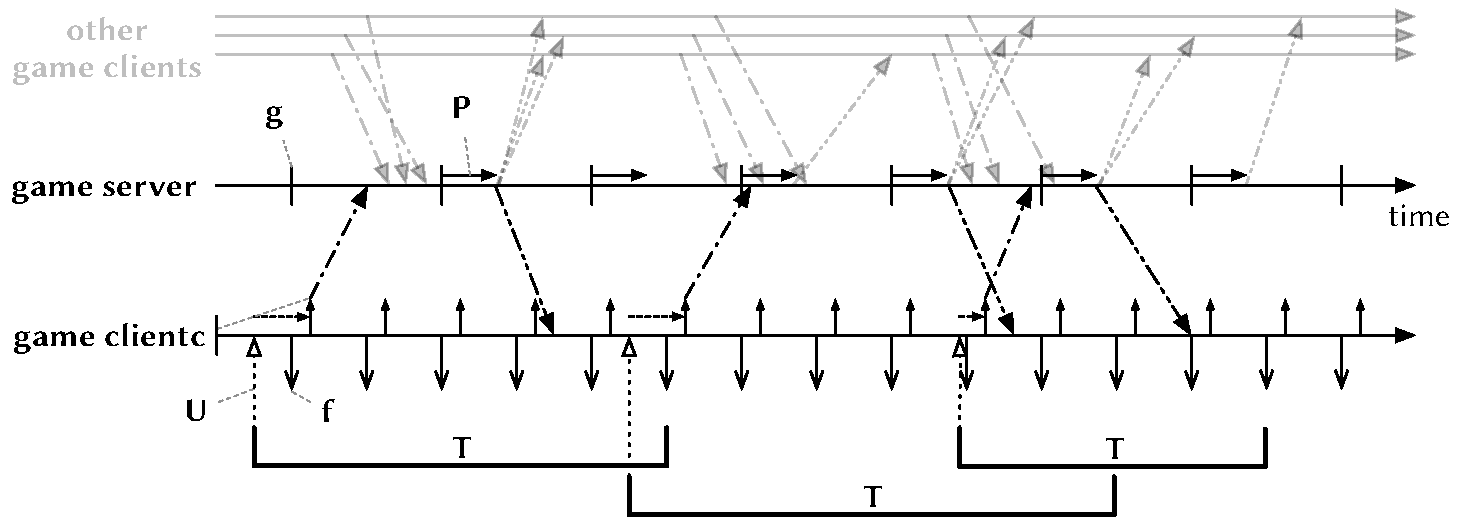
\includegraphics[width=1.0\columnwidth]{../../../models/tickrate-timeseries-notation.pdf}
% 	\caption{Exemplary flow of events in an online client-server game, and resulting end-to-end lag with the notation of Tab.~\ref{tab:notation}.
% 	% \hoss{Notation aus Tabelle ~\ref{tab:notation} waere gut im Bild. }
% 	} %Delay values are given for a framerate of \SI{60}{\hertz} and a server tickrate of \SI{30}{\hertz}, the network latency will only show minor variations.}
% \label{fig:tickrate-timeseries}
% \end{figure}



% \textbf{Factors in human perception and strategy}

% The models we present do not take into account the perceived lag from when the players \textit{think} they have triggered an action to when they perceive the outcomes of their action. This consequently disregards effects of different player actions, strategies, and so on.

